\documentclass[../thesis.tex]{subfiles}

\begin{document}

\section{Introduction\label{sec:int}}

Transport of inertial particles by turbulent flows is a common phenomenon observed in nature. The examples include dust storms, dunes formation, transport of organic matter in water reservoirs, or airborne particles, such as pollen, soot and ashes. Turbulent transport is also an important process in a variety of industrial applications, e.g.\ filtering of solid particles, propulsion systems, and oil processing. In this study, we focus on quantitative analysis of cloud microphysical processes in turbulent air. Accurate description of these complex atmospheric phenomena is central for reliable weather and climate predictions on Earth. Interaction of cloud droplets or ice crystals with the turbulent flow as well as interactions among different hydrometeors have a direct impact on the precipitation formation, i.e.\ the rate and amount of precipitation. The characteristic length scales of these microphysical processes are significantly smaller than those defining large-scale atmospheric flows; therefore, they cannot be resolved in numerical weather prediction (NWP) models. Nowadays, NWP models provide regular forecasts at horizontal resolutions varying from coarse resolutions of several kilometers up to one kilometer \citep{YZCTOBCDDG18}. In the standard NWP approach, the effect of cloud processes at unresolved scales is usually accounted for by parametrization, representing only some statistical features of the modeled systems. To develop more realistic parametrizations, a detailed knowledge of the physics underlying these processes is necessary.

The importance of the cloud microphysical process resulted in a rich scientific literature with a particular focus on quantifying the growth of cloud droplets in the sizes ranging from 10 to 60~$\mu$m in radius. This range is commonly called the size gap, for which neither the condensation nor the gravitational collision--coalescence mechanism is effective \citep{PK97, CYBX18}. A number of studies have been carried out to explain the growth of such droplets as well as the fast broadening of their size spectra. In these studies several mechanisms have been investigated such as growth by ultragiant particles \citep{VC07,YLRT00}, entrainment-induced spectral broadening \citep{B93}, effects of pre-existing clouds, and enhanced collision rate by turbulence \citep{GW13,DBBCGIMRVW12,RPAGW13}. In recent years, the most intensely analyzed and discussed is the mechanism of turbulent collision--coalescence \citep{GW13,RWMG11,RPAGW13,WARG08,RPAW16}.

Air turbulence can increase the rate of droplet collisions in several different ways. It can raise the probability of collisions by increasing the relative velocity between droplet pairs as a result of shear effects and differential acceleration. In addition, droplet trajectories are biased towards the regions of lower vorticity and higher strain rate. Consequently, turbulence can increase, in average, the clustering in the distribution of droplets, thus bringing droplets closer together and increasing the probability of collision. Moreover, if the effect of gravity is taken into consideration, the interaction of particles with the turbulent flow will selectively alter their settling velocity, consequently enhancing the collision rate. Furthermore, turbulence affects the local aerodynamic interactions among particles by changing their relative motion, local acceleration, and shear effects. 

In most previous numerical studies of cloud processes, the continuous phase was modeled using the Eulerian approach, employing direct numerical simulations (DNS) or large-eddy simulations (LES), e.g.\ \cite{RP17}, while the dispersed phase was treated using the Lagrangian approach together with the point-particle assumption and one-way momentum coupling between the continuous and dispersed phases \citep{RPAGW13,WRGHJ09}. This simplified approach will be sufficient only if the particles do not significantly affect the motion of the continuous phase. For larger concentrations, i.e.\ mass loadings, of the dispersed phase, the effect of turbulence modulation induced by particles becomes important. There are several studies where the effect of two-way momentum coupling was considered \citep{BKM06,MD17,RPW20,RPW20corrigendum}. It should be emphasized, however, that the effect of aerodynamic interaction in simulations with two-way coupling has been considered only to a limited extent. Full representation of lubrication forces, to the best of our knowledge, has so far never been included into the particle equations of motion. As for the fully resolved simulations of turbulence with finite-size particles, the two-way momentum coupling and particle aerodynamic interactions are automatically accounted for. Such studies have become possible only in recent years \citep{DBBCGIMRVW12,GLW13,K16,WPGY16-2,WPGY16}, yet, they are limited to a relatively small number of particles, typically of \textit{O}($10^5$).

An innovative method for treating the aerodynamic interactions among cloud droplets was introduced by \cite{WAG05}. Their improved superposition method (ISM) was tested in a set of idealized experiments aimed at computing the collision efficiency of small water droplets settling under gravity in stagnant air. Compared to the original superposition method \citep{PK97}, ISM is more accurate. For example, in simulations where the effect of lubrication is not dominant the relative error in the drag force can be reduced by an order of magnitude. The original formulation of the superposition method fails to satisfy the no-slip boundary condition on the surfaces of the interacting spheres, therefore errors in the representations of drag forces can be large. Application of ISM to a many-body system of mutually interacting droplets in a turbulent flow is rather straightforward, leading to the hybrid direct numerical simulation (HDNS) approach introduced by \cite{AGW07}. The basic idea of HDNS is to combine the DNS of the background turbulence with an analytical representation of the disturbance flows introduced by particles. This approach takes advantage of the fact that the disturbance flows due to droplets are localized in space and there is a sufficient length-scale separation between the droplet size and the Kolmogorov scale of the background flow. In HDNS, the disturbance flow experienced by each droplet due to the presence of other droplets is derived from a linear system of $3N_\text{p}$ unknowns, namely three components of velocity in each spatial direction, where $N_\text{p}$ is the number of droplets in the simulation. HDNS is a significant step forward in modeling cloud processes. Nevertheless, the iterative solution of the large linear system is computationally expensive.

The first HDNS implementation was developed based on OpenMP parallel library \citep{AGW07} and therefore it could not take the full advantage of modern machines with distributed memory. This limited the scalability of the code, and hence, the simulations could be run using low-resolution meshes, equivalent to low Reynolds numbers, and small numbers of particles. To increase the scalability of HDNS several attempts have been made \citep{RW09, RPAWG11c, RPAWG11p, APCRW14}, the most recent of which \citep{TPARW13} is a massively parallel implementation based on 2D domain decomposition that uses MPI library for data communication. Under HDNS framework, \cite{OTV13} proposed a more efficient approach named binary interaction-based superposition method suitable for dilute systems. Compared to HDNS, calculating the hydrodynamic interactions in systems typical of atmospheric clouds requires an order of magnitude less CPU time. Therefore, the method is capable of performing simulations with larger number of particles and using larger domains. As for the accuracy of the method, the error is comparable to that of HDNS if the volume fraction of the disperse phase is low. 

All the above-mentioned methods are based on the Stokes solution for a single sphere and therefore cannot correctly handle short-range or lubrication forces. Other studies in which the simple superposition method was used \citep{SN63, SG71, LL75, PKS01} resulted in a rough prediction of the collision efficiency. Therefore, rigorously incorporating the lubrication effect is necessary in order to obtain reliable data to quantify the microphysical processes.

There are several studies aimed at investigating the lubrication forces between spherical particles. The first rigorous analytical solution for an idealized system of two coaxial spheres moving at equal small constant velocities along their line of centers was developed by \cite{SJ26}. Another interesting example, here, is the solution elaborated by \cite{JO84}. They considered an unbounded low-Reynolds-number viscous flow enforced by translational and rotational motion of two unequal rigid spheres. The forces and torques acting on the particles were derived in terms of an infinite series making use of the twin multipole expansions method. While relatively easy for numerical implementation, their solutions are valid for all separation distances between spheres and accurately represent the asymptotic behavior of the forces when the gap distance between them goes to zero, i.e.\ the lubrication effects. Very recently, \cite{GMS20} used a bipolar coordinate system to develop an alternative representation of interacting forces for a squeezing flow of two unequal rigid spheres and a shearing flow of two equal-sized spheres. They claimed that for different size particles their solution is more precise comparing to the asymptotic solutions of other existing methods. There are also some studies in which lubrication interactions among three spherical particles are considered, e.g.\ \cite{CEW99}. Also, the dynamics as well as stability of three spheres sedimenting under gravity was examined by \cite{EW06}. Unfortunately, the computational cost of such simulations is so large that the method cannot be directly used for modeling systems with many particles.

\cite{RWMG11} developed a computationally efficient approach for treating the aerodynamic interactions between two spheres moving in still air. Compared with the exact solution of \cite{JO84}, the forces and torques were accurately represented in the entire range of separation distances. The method combines the Force--Torque--Stresslet (FTS) multipole expansion of \cite{DBB87} for the long-range interaction with the lubrication expansion of \cite{JO84} at short separation distances. For the intermediate range where no simple method is available, a third-order polynomial fitting was used to bridge the treatments for long-range and short-range interactions. This composite approach resulted in a large reduction in the computational cost when compared to the full treatment of \cite{JO84}, while keeping the relative error in calculated collision efficiency typically within only \textit{O}($1\%$). This approach, while numerically efficient, allows to handle the interaction between two particles, not among many particles. Hence, further advancement is needed in order to adopt the method for computing collision statistics of many droplets in turbulent flows.

Accordingly, the objective of this study is to investigate dynamics of cloud droplets under one-way momentum coupling in homogeneous isotropic turbulence (HIT), considering full representation of interaction forces, i.e.\ including the effects of lubrication. To achieve this goal, the exact analytical solution developed by \cite{JO84} has been incorporated into the numerical code for HDNS. The simulations of turbulent flows are handled using the standard pseudo-spectral method, as detailed in Section 2. The hybrid approach is rigorous and convenient for studying collision statistics, preferential concentration, and collision efficiency of cloud droplets.

The content of this paper is structured as follows. In Section 2, we describe the numerical tools that are used to simulate homogeneous isotropic turbulence and particle tracking. Results from HDNS are discussed in Section 3. These include sensitivity of the kinematic and dynamic collision statistics to the time step size and location of matching point. This matching point indicates the separation distance at which standard HDNS switches to short-range analytical solution. Extended analysis of the radial distribution function (RDF) and radial relative velocity (RRV) at different droplet mass loadings is presented in Section 4. Section 5 contains a summary and main conclusions.

%%%%%%%%%%%%% I N T R O D U C T I O N %%%%%%%%%%%
\paragraph{PPAM}
Particle-laden turbulent flows are present in a large number of industrial and natural processes such as fuel combustion, dispersion of pollution by air, or sediment transport in water. In clouds, turbulence is the main cause of collision--coalescence of rain drops within the radii range $10$--$60~\mu$m. This results in droplets growing and eventually initiates rainfall.

Simulating microphysical processes in clouds entails enormous computational costs due to the wide range of length and time scales associated with turbulent flows and the consideration of aerodynamic interactions among a large number of particles. Thanks to development of modern high-performance computing techniques, such simulations are feasible within a reasonable time. The standard approach to model cloud processes is based on an Eulerian--Lagrangian description. It employs the direct numerical simulations (DNS) for simulating the turbulent flow. Droplet tracking is carried out by integrating their individual trajectories \cite{WM93}. DNS handles the evolution of the turbulent field resolving all scales of the flow down to the smallest (i.e.~Kolmogorov) ones. The locations of the droplets in the domain are updated at every time step, and therefore the numerical cost is proportional to the number of particles in the domain.

Aerodynamic interaction among the particles can be accounted for via ``superposing'' the disturbance velocity fields induced around every single particle due to its motion in a viscous medium \cite{WAG05}. This results in a very large system of equations for three components of disturbance velocities at the location of every particle generated by its neighboring particles \cite{AGW07}. Consequently, solving such a large system substantially adds to the computational cost of simulations \cite{APCRW14}. In the literature, the combination of DNS for the background turbulent field and this analytical representation of interaction is known as hybrid DNS. HDNS by itself, however, is unable to capture short-range viscous forces, known as lubrication interactions, acting on particles \cite{WAG05}. Once the distance between particles is comparable to their average radii, superposition of their disturbances does not yield the accurate force, because the superposition method is based on the solution to the Stokes flow around a single sphere. Thus, the representation of aerodynamic interaction can be improved by utilizing HDNS \cite{AGW07} for distant particles together with exact analytical solutions \cite{JO84} for particles in proximity.

The physics of this model has already been investigated \cite{ARPW21}, but a quantitative evaluation of the computational aspects remains to be addressed. Furthermore, it has been shown that without lubrication effects simulation time increases with the number of droplets in the domain \cite{APCRW14}, but it is expected that considering lubrication reduces this time. This is because for the particles in proximity short-range interaction is considered, thereby excluding such pairs from the matrix of disturbances for AI. As a result, a smaller matrix needs to be inverted which is less demanding. In addition, the size of the distance below (over) which the lubrication effect (superposed disturbances) would be considered is another key factor affecting computation time. Moreover, it is important to address the scalability of this implementation with the number of CPU cores. Additionally, we want to check the feasibility and evaluate the cost of simulations with higher resolution meshes and larger liquid water contents (LWC). The aim of this study is to assess all these aspects of the model by making use of data from numerical simulations.


\begin{figure}
\center
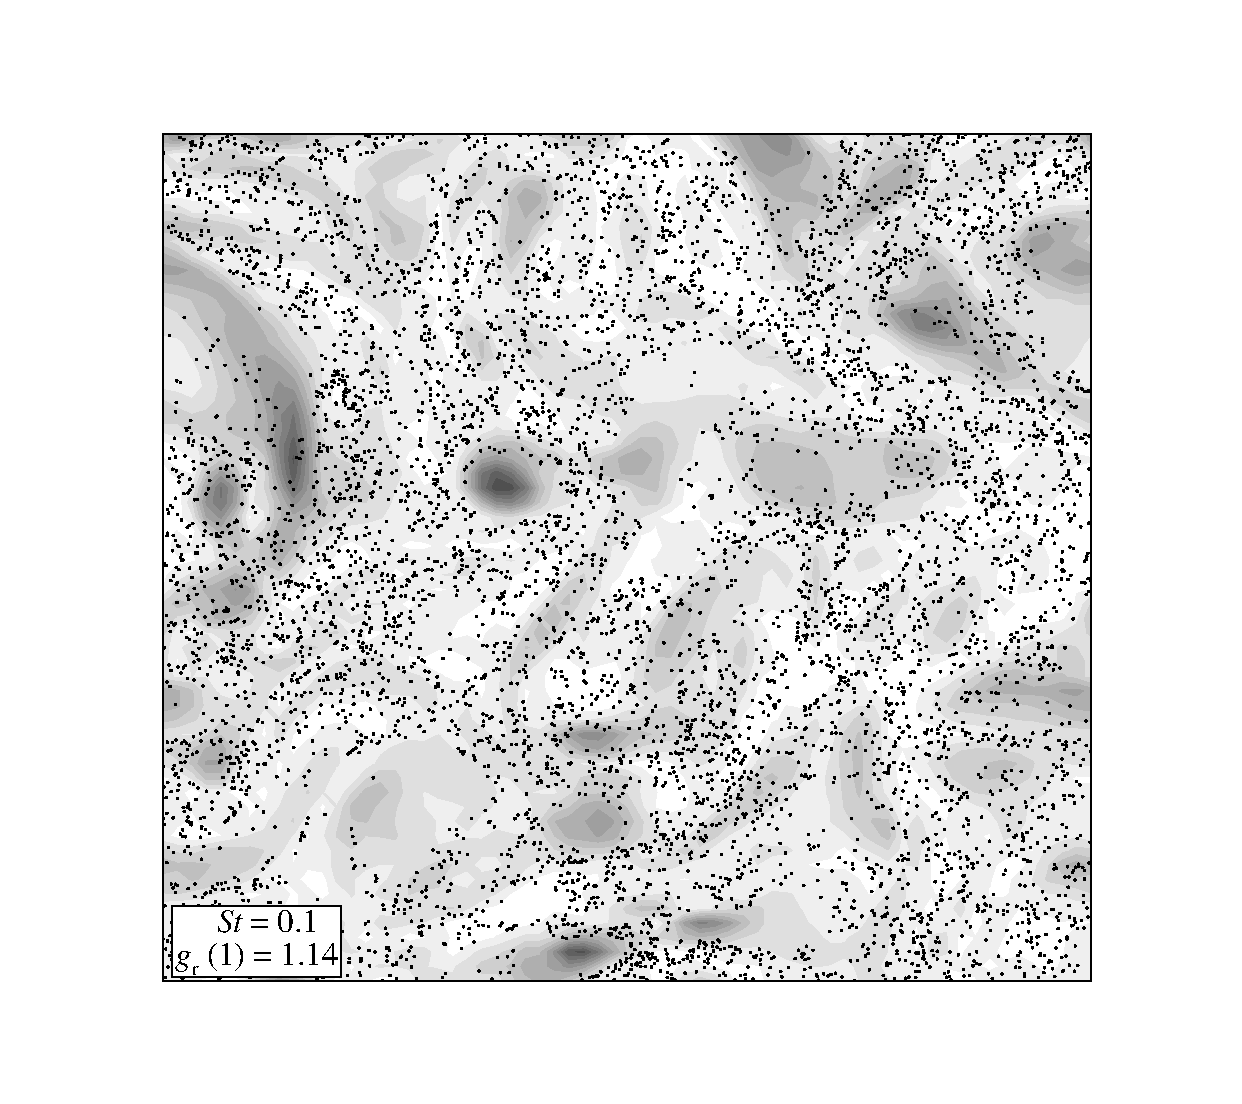
\includegraphics[trim=27mm 20mm 25mm 21mm, clip, width=0.49\textwidth]{../figs/Pref-conc/St = 0.1.pdf}
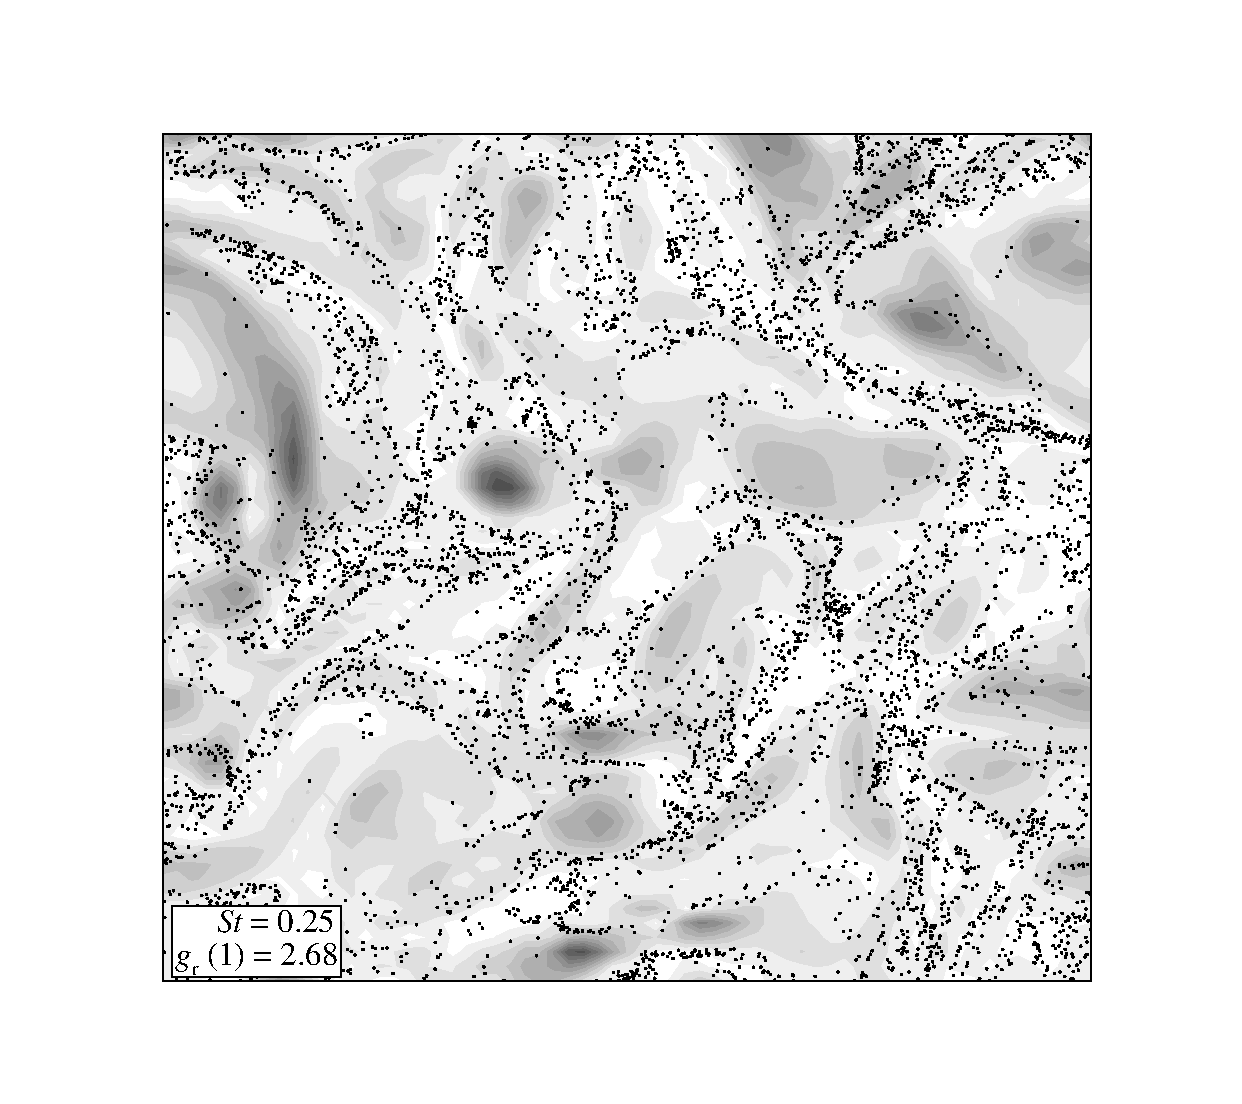
\includegraphics[trim=27mm 20mm 25mm 21mm, clip, width=0.49\textwidth]{../figs/Pref-conc/St = 0.25.pdf}
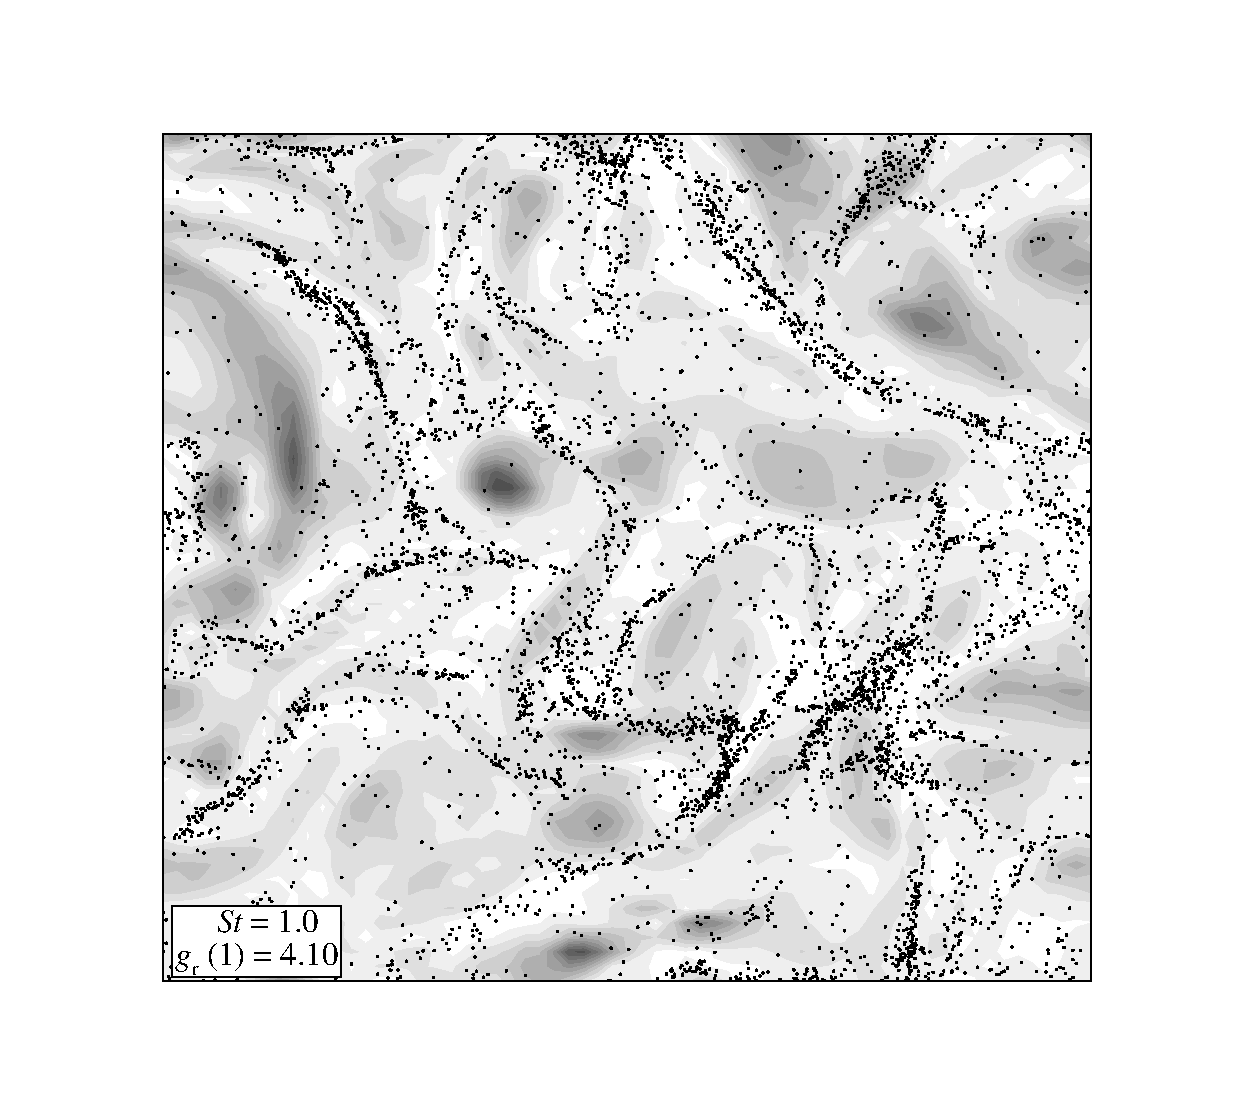
\includegraphics[trim=27mm 20mm 25mm 21mm, clip, width=0.49\textwidth]{../figs/Pref-conc/St = 1.pdf}
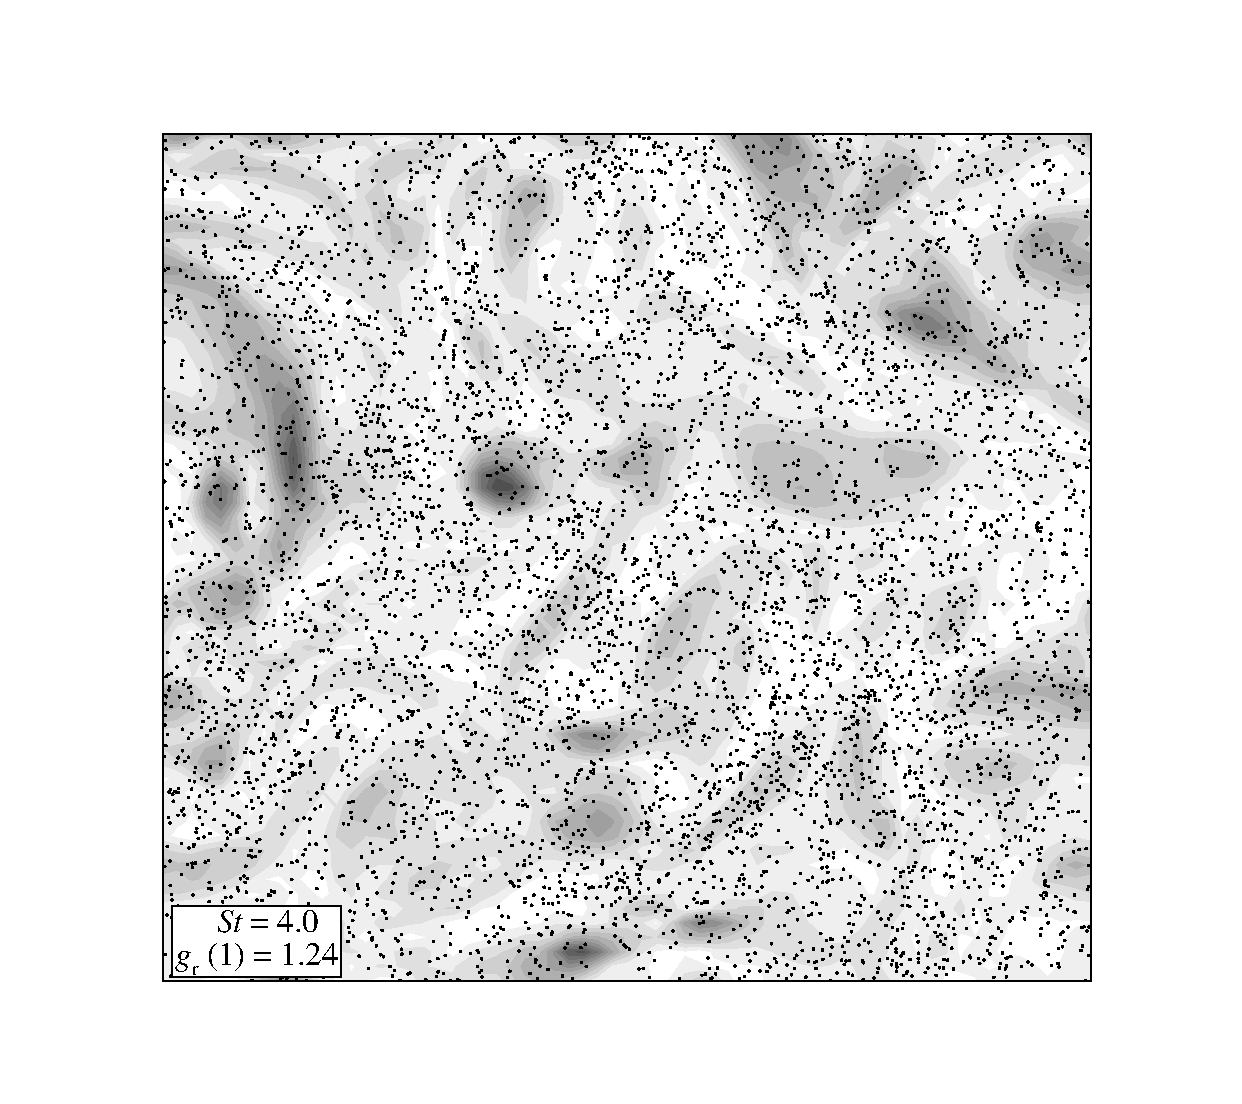
\includegraphics[trim=27mm 20mm 25mm 21mm, clip, width=0.49\textwidth]{../figs/Pref-conc/St = 4.pdf}
\caption{Preferential concentration}
\label{fig:pref}
\end{figure}

%\bibliographystyle{bibstyle}
%\bibliography{references}
\newpage
\end{document}
